\section{Results}\label{sec:results}

\begin{table*}[t]
\centering
\scriptsize
\caption{Main results: test AUC and DPD (mean $\pm$ sd over seeds). Best per column in bold. $^\dagger$: Holm-adjusted Wilcoxon signed-rank $p<0.05$ against CLAMP, paired by seed.}
\setlength{\tabcolsep}{2pt}
\begin{minipage}[t]{0.49\textwidth}
\centering
\begin{tabular}{l cc cc cc cc}
\toprule
 & \multicolumn{2}{c}{German} & \multicolumn{2}{c}{Bail} & \multicolumn{2}{c}{Credit} & \multicolumn{2}{c}{Pokec-z} \\
 & AUC & DPD & AUC & DPD & AUC & DPD & AUC & DPD \\
\midrule
FedAvg-GAT & \textbf{0.76$\pm$0.05} & 0.11$\pm$0.06 & 0.80$\pm$0.04 & 0.02$\pm$0.01 & 0.77$\pm$0.01 & 0.08$\pm$0.01$^\dagger$ & 0.74$\pm$0.02 & 0.03$\pm$0.01 \\
FairFed & 0.75$\pm$0.05 & 0.05$\pm$0.04 & \textbf{0.80$\pm$0.03} & 0.01$\pm$0.01 & 0.75$\pm$0.01 & 0.01$\pm$0.01 & 0.64$\pm$0.05$^\dagger$ & \textbf{0.00$\pm$0.00}$^\dagger$ \\
F2GNN & 0.73$\pm$0.02 & 0.04$\pm$0.03 & 0.78$\pm$0.03 & 0.01$\pm$0.01 & 0.76$\pm$0.01 & \textbf{0.01$\pm$0.01} & 0.74$\pm$0.02 & 0.01$\pm$0.01$^\dagger$ \\
FairGFL & 0.74$\pm$0.05 & 0.08$\pm$0.07 & 0.78$\pm$0.03 & 0.01$\pm$0.01 & 0.76$\pm$0.01 & 0.07$\pm$0.01$^\dagger$ & 0.66$\pm$0.02$^\dagger$ & 0.04$\pm$0.01 \\
FedGraph-Fair & 0.66$\pm$0.09 & 0.08$\pm$0.05 & 0.76$\pm$0.03 & 0.01$\pm$0.01 & 0.75$\pm$0.01 & 0.08$\pm$0.01$^\dagger$ & 0.64$\pm$0.03$^\dagger$ & 0.04$\pm$0.01 \\
FedFACT & 0.72$\pm$0.04 & 0.08$\pm$0.06 & 0.80$\pm$0.03 & 0.01$\pm$0.01 & 0.75$\pm$0.01 & 0.07$\pm$0.02$^\dagger$ & 0.63$\pm$0.04$^\dagger$ & 0.02$\pm$0.01 \\
PUFFLE & 0.49$\pm$0.08$^\dagger$ & \textbf{0.01$\pm$0.01} & 0.50$\pm$0.06$^\dagger$ & \textbf{0.00$\pm$0.00} & 0.46$\pm$0.13$^\dagger$ & 0.02$\pm$0.01 & 0.55$\pm$0.11$^\dagger$ & 0.01$\pm$0.01$^\dagger$ \\
FedFDP & 0.53$\pm$0.09$^\dagger$ & 0.01$\pm$0.02 & 0.51$\pm$0.03$^\dagger$ & 0.00$\pm$0.00$^\dagger$ & 0.54$\pm$0.11$^\dagger$ & 0.02$\pm$0.01 & 0.64$\pm$0.11$^\dagger$ & 0.01$\pm$0.01$^\dagger$ \\
FairGNN & 0.57$\pm$0.06$^\dagger$ & 0.11$\pm$0.08 & 0.56$\pm$0.09$^\dagger$ & 0.02$\pm$0.02 & 0.67$\pm$0.09$^\dagger$ & 0.10$\pm$0.06 & 0.54$\pm$0.08$^\dagger$ & 0.01$\pm$0.01 \\
FairSIN & 0.72$\pm$0.05 & 0.09$\pm$0.06 & 0.79$\pm$0.03 & 0.02$\pm$0.01$^\dagger$ & 0.75$\pm$0.00 & 0.07$\pm$0.01$^\dagger$ & 0.66$\pm$0.05$^\dagger$ & 0.03$\pm$0.01 \\
ClipMean (no controller, last iterate) & 0.73$\pm$0.06 & 0.09$\pm$0.07 & 0.78$\pm$0.03 & 0.02$\pm$0.01 & \textbf{0.77$\pm$0.01} & 0.07$\pm$0.01$^\dagger$ & 0.75$\pm$0.02 & 0.04$\pm$0.01$^\dagger$ \\
CLAMP (last iterate) & 0.73$\pm$0.07 & 0.05$\pm$0.05 & 0.78$\pm$0.03 & 0.02$\pm$0.01 & 0.76$\pm$0.01 & 0.05$\pm$0.05 & 0.75$\pm$0.02 & 0.03$\pm$0.00 \\
CLAMP-Select (no controller) & 0.71$\pm$0.09 & 0.07$\pm$0.07 & 0.78$\pm$0.03 & 0.02$\pm$0.01 & 0.72$\pm$0.15 & 0.06$\pm$0.02 & \textbf{0.77$\pm$0.03} & 0.03$\pm$0.01 \\
\textbf{CLAMP} & 0.71$\pm$0.08 & 0.05$\pm$0.05 & 0.78$\pm$0.03 & 0.02$\pm$0.01 & 0.76$\pm$0.01 & 0.02$\pm$0.01 & 0.75$\pm$0.02 & 0.03$\pm$0.00 \\
CLAMP-GCN & 0.71$\pm$0.11 & 0.06$\pm$0.05 & 0.79$\pm$0.02 & 0.01$\pm$0.01 & 0.75$\pm$0.01 & 0.01$\pm$0.01 & 0.72$\pm$0.02$^\dagger$ & 0.03$\pm$0.01 \\
\bottomrule
\end{tabular}
\end{minipage}\hfill
\begin{minipage}[t]{0.49\textwidth}
\centering
\begin{tabular}{l cc cc cc cc}
\toprule
 & \multicolumn{2}{c}{Pokec-n} & \multicolumn{2}{c}{AMiner-S} & \multicolumn{2}{c}{NBA} & \multicolumn{2}{c}{Facebook} \\
 & AUC & DPD & AUC & DPD & AUC & DPD & AUC & DPD \\
\midrule
FedAvg-GAT & 0.75$\pm$0.02 & 0.03$\pm$0.02 & 0.94$\pm$0.00 & 0.01$\pm$0.00$^\dagger$ & \textbf{0.81$\pm$0.06} & 0.10$\pm$0.06 & 0.77$\pm$0.05 & 0.08$\pm$0.05 \\
FairFed & 0.62$\pm$0.06$^\dagger$ & 0.01$\pm$0.00$^\dagger$ & 0.94$\pm$0.00 & 0.00$\pm$0.00 & 0.80$\pm$0.05 & 0.08$\pm$0.06 & 0.76$\pm$0.03 & 0.05$\pm$0.03 \\
F2GNN & 0.74$\pm$0.03$^\dagger$ & 0.01$\pm$0.01$^\dagger$ & \textbf{0.94$\pm$0.01}$^\dagger$ & 0.01$\pm$0.00 & 0.78$\pm$0.13 & 0.11$\pm$0.07 & 0.76$\pm$0.05 & 0.07$\pm$0.04 \\
FairGFL & 0.65$\pm$0.03$^\dagger$ & 0.04$\pm$0.01$^\dagger$ & 0.94$\pm$0.01 & 0.00$\pm$0.00 & 0.76$\pm$0.04 & 0.08$\pm$0.04 & 0.75$\pm$0.05 & 0.08$\pm$0.04 \\
FedGraph-Fair & 0.59$\pm$0.05$^\dagger$ & 0.02$\pm$0.01 & 0.93$\pm$0.01$^\dagger$ & 0.00$\pm$0.00 & 0.77$\pm$0.10 & 0.08$\pm$0.04 & 0.74$\pm$0.05 & 0.09$\pm$0.04 \\
FedFACT & 0.59$\pm$0.06$^\dagger$ & 0.01$\pm$0.01 & 0.92$\pm$0.01$^\dagger$ & 0.01$\pm$0.00 & 0.76$\pm$0.04 & 0.14$\pm$0.08 & 0.74$\pm$0.05 & 0.05$\pm$0.04 \\
PUFFLE & 0.57$\pm$0.11$^\dagger$ & 0.01$\pm$0.01 & 0.49$\pm$0.03$^\dagger$ & 0.01$\pm$0.00 & 0.37$\pm$0.19 & \textbf{0.01$\pm$0.01} & 0.53$\pm$0.10$^\dagger$ & \textbf{0.01$\pm$0.01} \\
FedFDP & 0.66$\pm$0.08$^\dagger$ & 0.01$\pm$0.01 & 0.49$\pm$0.03$^\dagger$ & 0.01$\pm$0.00 & 0.39$\pm$0.20$^\dagger$ & 0.02$\pm$0.01$^\dagger$ & 0.54$\pm$0.08 & 0.01$\pm$0.01 \\
FairGNN & 0.50$\pm$0.00$^\dagger$ & \textbf{0.00$\pm$0.00}$^\dagger$ & 0.63$\pm$0.08$^\dagger$ & 0.10$\pm$0.04$^\dagger$ & 0.77$\pm$0.08 & 0.10$\pm$0.04 & 0.51$\pm$0.05 & 0.02$\pm$0.04 \\
FairSIN & 0.64$\pm$0.06$^\dagger$ & 0.04$\pm$0.01 & 0.92$\pm$0.01$^\dagger$ & 0.00$\pm$0.00 & 0.73$\pm$0.08 & 0.09$\pm$0.06 & 0.74$\pm$0.05 & 0.07$\pm$0.03 \\
ClipMean (no controller, last iterate) & 0.75$\pm$0.02 & 0.05$\pm$0.02$^\dagger$ & 0.94$\pm$0.01 & 0.00$\pm$0.00 & 0.78$\pm$0.08 & 0.09$\pm$0.07 & 0.77$\pm$0.06 & 0.09$\pm$0.04 \\
CLAMP (last iterate) & 0.75$\pm$0.02 & 0.03$\pm$0.01 & 0.94$\pm$0.01 & 0.00$\pm$0.00 & 0.79$\pm$0.07 & 0.09$\pm$0.07 & \textbf{0.77$\pm$0.06} & 0.08$\pm$0.04 \\
CLAMP-Select (no controller) & 0.76$\pm$0.03 & 0.03$\pm$0.01 & 0.94$\pm$0.01 & 0.00$\pm$0.00 & 0.79$\pm$0.09 & 0.06$\pm$0.05 & 0.75$\pm$0.09 & 0.08$\pm$0.04 \\
\textbf{CLAMP} & \textbf{0.76$\pm$0.02} & 0.03$\pm$0.01 & 0.94$\pm$0.01 & 0.00$\pm$0.00 & 0.80$\pm$0.08 & 0.08$\pm$0.05 & 0.75$\pm$0.09 & 0.07$\pm$0.04 \\
CLAMP-GCN & 0.71$\pm$0.02$^\dagger$ & 0.03$\pm$0.01 & 0.94$\pm$0.00 & \textbf{0.00$\pm$0.00} & 0.78$\pm$0.07 & 0.08$\pm$0.04 & 0.72$\pm$0.13 & 0.07$\pm$0.04 \\
\bottomrule
\end{tabular}
\end{minipage}
\label{tab:e1_main_compact}
\end{table*}


\subsection{Fairness and utility}\label{sec:main}

Table~\ref{tab:e1_main_compact} reports test AUC and $\dpd$ for all methods on the eight datasets; the full table with $\eod$, the selected round and the certificate of Proposition~\ref{prop:cert} is in the supplementary material. We read it in three groups.

\paragraph{Where the budget binds}
On Credit, Pokec-z and Pokec-n the unconstrained clipped model (ClipMean) has a gap above the budget $\tau=0.03$ (0.071, 0.042 and 0.052). \clamp{} brings it to 0.018, 0.026 and 0.028 at essentially the same AUC as ClipMean (0.76, 0.75 and 0.76 against 0.77, 0.75 and 0.75). The test gap is at or below $\tau$ for 8, 9 and 5 of the 10 seeds; the remaining seeds exceed it on test data although the returned model met the budget on validation data, which is the validation--test generalisation gap that Proposition~\ref{prop:output} does not cover. The baselines that read per-client fairness or group rates in the clear reach lower gaps: F$^2$GNN 0.006--0.008 at AUC 0.74--0.76, and FairFed 0.004--0.008, but at a large AUC cost on the Pokec graphs (0.62--0.64). \clamp{} is not designed to drive the gap to zero; it holds it at the budget the federation chooses, and Section~\ref{sec:tau} shows that lower budgets are reachable. FairGFL, FedGraph-Fair, FedFACT and FairSIN leave the gap close to that of FedAvg on these datasets. The two private methods, PUFFLE and FedFDP, have small gaps only because they barely learn: with gradient noise at $\varepsilon=8$ their AUC is between 0.46 and 0.65 on every dataset.

\paragraph{Where the budget does not bind}
On Bail and AMiner-S the unconstrained gap is already below $\tau$ (0.016 and 0.005), so the multiplier stays at zero, \clamp{} coincides with ClipMean, and all reasonable methods are within noise of each other.

\paragraph{Small graphs}
On German, NBA and Facebook (403 to 1{,}045 nodes) every method has a large seed-to-seed spread, and \clamp{} improves only modestly on ClipMean (German 0.088 to 0.058, NBA 0.093 to 0.076, Facebook 0.086 to 0.069), and in 2 to 4 of 10 runs no release round after the warm-up was feasible, so the output rule fell back to the last model. With a few dozen validation nodes per group and client, the noisy statistics are a weak signal even with $P=10$ (Section~\ref{sec:privacy}), and the validation gap is a poor proxy for the test gap.

\paragraph{The output rule}
The rows labelled ``last iterate'' return the final model instead of the stored feasible one. On Credit this changes the mean gap from 0.018 to 0.055 and its standard deviation from 0.015 to 0.046: the signed penalty makes the gap oscillate around the budget, and the last iterate lands anywhere on the oscillation. Selection without the controller (\clamp{}-Select, $\eta=0$) does not reproduce the effect: its gap is 0.067, 0.041 and 0.052 on Credit, Pokec-z and Pokec-n, close to ClipMean, and it finds an eligible feasible round in only 7, 2 and 1 of 10 runs. The controller creates feasible models and the output rule picks one. On Credit and the Pokec graphs the selected round is late (98--99 on average), so the returned model has been trained almost as long as the last one.

\subsection{Controllability of the fairness budget}\label{sec:tau}

\begin{figure}[t]
\centering
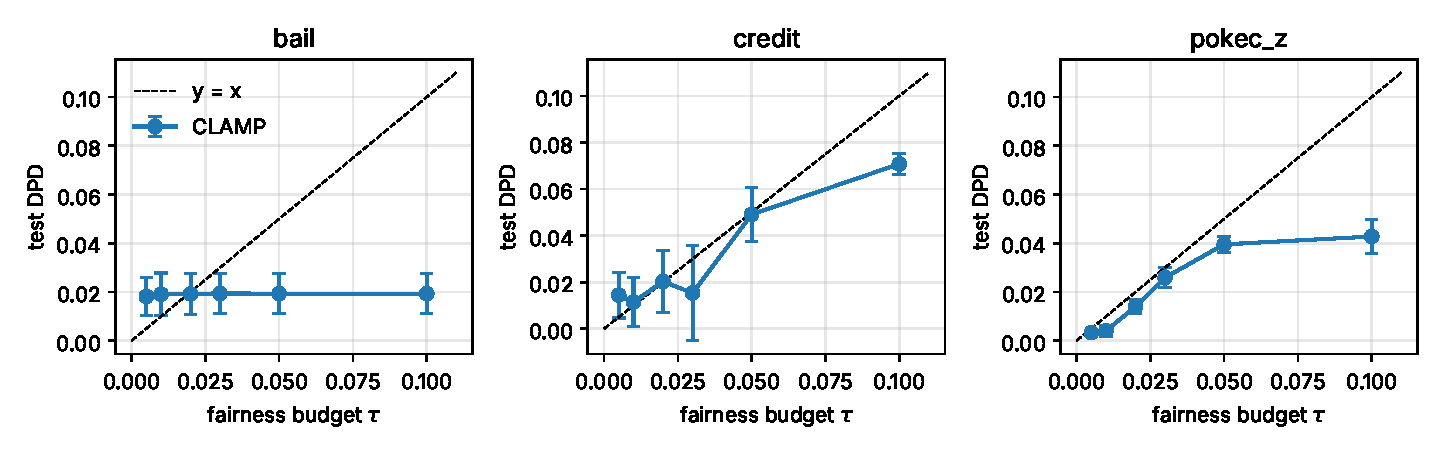
\includegraphics[width=0.6\linewidth]{figures/e2_tau_pareto}
\caption{Test $\dpd$ of \clamp{} against the budget $\tau$ (mean over five seeds; dashed: $\dpd=\tau$).}\label{fig:tau}
\end{figure}

Figure~\ref{fig:tau} varies $\tau$ from 0.005 to 0.1. On Pokec-z the test gap follows the budget closely (0.003, 0.004, 0.014, 0.026, 0.040 and 0.043 for the six values) while AUC stays between 0.741 and 0.746. On Credit the gap is 0.012--0.020 for every $\tau\le0.03$, rises to 0.049 at $\tau=0.05$ and reaches the unconstrained 0.071 at $\tau=0.1$; tightening the budget costs about 0.02 AUC (0.773 to 0.753). On Bail the gap stays at 0.018--0.019 for every budget: the test gap of this dataset is not reduced by the controller even at $\tau=0.005$, and the tighter budget costs AUC (Section~\ref{sec:privacy}). A single protocol parameter therefore sets the operating point on the two datasets where the constraint is informative, and at $\tau=0.005$ \clamp{} on Pokec-z matches the gap of the best baseline (F$^2$GNN, 0.008) at a higher AUC (0.746 against 0.739).

\subsection{Byzantine updates}\label{sec:byz}
% E3 results are inserted when the attack campaign completes.

\subsection{Falsified statistics}\label{sec:statattack}

\begin{table}[t]
\centering
\small
\caption{Statistics attacks: deviation of the server's estimate from the honest-only gap, against the Theorem 3 bound plus the statistics-noise term (beta = 0.05). Violation counts are over all checked rounds and seeds.}
\begin{tabular}{llllllllll}
\toprule
dataset & attack & b & runs & rounds checked & max\_t |dhat-D^H| & max\_t bound (b-term + noise) & rounds violating bound & AUC & DPD \\
\midrule
bail & none & 0 & 3 & 300 & 0.017 & 0.070 & 0 & 0.745 ± 0.017 & 0.009 ± 0.003 \\
bail & stat\_falsify & 1 & 3 & 300 & 0.014 & 0.512 & 0 & 0.745 ± 0.017 & 0.009 ± 0.003 \\
bail & stat\_falsify & 2 & 3 & 300 & 0.015 & 0.956 & 0 & 0.745 ± 0.017 & 0.010 ± 0.003 \\
bail & stat\_falsify & 3 & 3 & 300 & 0.014 & 1.230 & 0 & 0.745 ± 0.017 & 0.009 ± 0.003 \\
bail & stat\_falsify & 4 & 3 & 300 & 0.011 & 1.429 & 0 & 0.745 ± 0.017 & 0.009 ± 0.003 \\
bail & stat\_falsify\_mid & 1 & 3 & 300 & 0.014 & 0.512 & 0 & 0.745 ± 0.017 & 0.009 ± 0.003 \\
bail & stat\_falsify\_mid & 2 & 3 & 300 & 0.014 & 0.956 & 0 & 0.745 ± 0.017 & 0.010 ± 0.003 \\
bail & stat\_falsify\_mid & 3 & 3 & 300 & 0.014 & 1.230 & 0 & 0.745 ± 0.017 & 0.009 ± 0.003 \\
bail & stat\_falsify\_mid & 4 & 3 & 300 & 0.011 & 1.429 & 0 & 0.745 ± 0.017 & 0.009 ± 0.003 \\
pokec\_z & none & 0 & 3 & 300 & 0.006 & 0.021 & 0 & 0.764 ± 0.003 & 0.028 ± 0.016 \\
pokec\_z & stat\_falsify & 1 & 3 & 300 & 0.028 & 0.562 & 0 & 0.765 ± 0.002 & 0.045 ± 0.008 \\
pokec\_z & stat\_falsify & 2 & 3 & 300 & 0.041 & 1.018 & 0 & 0.765 ± 0.002 & 0.044 ± 0.008 \\
pokec\_z & stat\_falsify & 3 & 3 & 300 & 0.037 & 1.266 & 0 & 0.765 ± 0.003 & 0.045 ± 0.008 \\
pokec\_z & stat\_falsify & 4 & 3 & 300 & 0.031 & 1.434 & 0 & 0.765 ± 0.002 & 0.045 ± 0.008 \\
pokec\_z & stat\_falsify\_mid & 1 & 3 & 300 & 0.016 & 0.562 & 0 & 0.763 ± 0.001 & 0.041 ± 0.007 \\
pokec\_z & stat\_falsify\_mid & 2 & 3 & 300 & 0.026 & 1.018 & 0 & 0.766 ± 0.003 & 0.046 ± 0.007 \\
pokec\_z & stat\_falsify\_mid & 3 & 3 & 300 & 0.031 & 1.266 & 0 & 0.765 ± 0.002 & 0.045 ± 0.009 \\
pokec\_z & stat\_falsify\_mid & 4 & 3 & 300 & 0.036 & 1.434 & 0 & 0.765 ± 0.002 & 0.045 ± 0.008 \\
credit & none & 0 & 3 & 300 & 0.051 & 0.141 & 0 & 0.756 ± 0.005 & 0.011 ± 0.004 \\
credit & stat\_falsify & 1 & 3 & 300 & 0.065 & 1.084 & 0 & 0.762 ± 0.005 & 0.064 ± 0.008 \\
credit & stat\_falsify & 2 & 3 & 300 & 0.058 & 1.391 & 0 & 0.762 ± 0.005 & 0.065 ± 0.008 \\
credit & stat\_falsify & 3 & 3 & 300 & 0.047 & 1.589 & 0 & 0.762 ± 0.005 & 0.064 ± 0.007 \\
credit & stat\_falsify & 4 & 3 & 300 & 0.092 & 1.805 & 0 & 0.621 ± 0.248 & 0.048 ± 0.032 \\
credit & stat\_falsify\_mid & 1 & 3 & 300 & 0.057 & 1.084 & 0 & 0.762 ± 0.005 & 0.065 ± 0.008 \\
credit & stat\_falsify\_mid & 2 & 3 & 300 & 0.059 & 1.391 & 0 & 0.762 ± 0.005 & 0.064 ± 0.008 \\
credit & stat\_falsify\_mid & 3 & 3 & 300 & 0.062 & 1.589 & 0 & 0.762 ± 0.005 & 0.064 ± 0.008 \\
credit & stat\_falsify\_mid & 4 & 3 & 300 & 0.063 & 1.805 & 0 & 0.762 ± 0.005 & 0.064 ± 0.008 \\
\bottomrule
\end{tabular}
\label{tab:e4_stat_attacks}
\end{table}


Table~\ref{tab:e4_stat_attacks} lets $b\in\{1,\dots,4\}$ of $K=10$ clients falsify their statistics. Two facts stand out. First, the bound of Theorem~\ref{thm:stats}, including its noise term, held: in every one of the 7{,}200 attacked rounds the observed deviation of the estimate from the honest gap was at most 0.092, against bounds between 0.51 and 1.81. The bound is valid but loose, because it allows every Byzantine client the full cap $\ncap$ in the smaller group. Second, the attack is effective where the budget binds. On Credit a single falsifying client out of ten raises the test gap of \clamp{} from 0.011 to 0.064, and on Pokec-z from 0.028 to 0.045. In both cases the gap returns to approximately the unconstrained level (ClipMean: 0.071 and 0.042) and AUC is unchanged: the adversary can switch the controller off. With four liars out of ten the swap attack does worse in one Credit run: the corrupted estimate drives the multiplier up, no round after the warm-up is feasible, and the returned last model has a gap of 0.46. A minority that controls the statistics can therefore not only disable fairness control but, through a runaway multiplier, damage the model it is meant to protect. The ``mid'' attack, which reports the honest pooled rate for both groups, is as effective as the swap attack. On Bail the attack has no effect because the controller is inactive there. Protecting the fairness channel against a small number of liars without seeing individual reports is the main open problem this work leaves (Section~\ref{sec:discussion}).

\subsection{Privacy}\label{sec:privacy}

\begin{table}[t]
\centering
\footnotesize
\caption{Differencing attack on the statistics channel: balanced accuracy of the likelihood-ratio test over random validation targets, mean$\pm$sd over seeds. Single: one noisy release. All: the $R$ releases of an unchanged vector ($R=10$ for German, $R=100$ for Bail), the worst case the theorem accounts for. Bound: $(e^{\varepsilon}+\delta)/(1+e^{\varepsilon})$. Monte Carlo and closed-form values agree to within 0.005.}
\label{tab:privacy_attack}
\begin{tabular}{lccccc}
\toprule
$\varepsilon$ & Bound & German single & German all & Bail single & Bail all \\
\midrule
1 & 0.731 & 0.513$\pm$0.003 & 0.542$\pm$0.003 & 0.504$\pm$0.001 & 0.537$\pm$0.001 \\
2 & 0.881 & 0.525$\pm$0.003 & 0.579$\pm$0.004 & 0.507$\pm$0.001 & 0.570$\pm$0.001 \\
4 & 0.982 & 0.547$\pm$0.003 & 0.644$\pm$0.004 & 0.513$\pm$0.001 & 0.629$\pm$0.001 \\
8 & 1.000 & 0.584$\pm$0.004 & 0.747$\pm$0.004 & 0.524$\pm$0.001 & 0.726$\pm$0.001 \\
16 & 1.000 & 0.645$\pm$0.004 & 0.878$\pm$0.003 & 0.541$\pm$0.001 & 0.854$\pm$0.001 \\
$\infty$ & 1.000 & 1.000$\pm$0.000 & 1.000$\pm$0.000 & 1.000$\pm$0.000 & 1.000$\pm$0.000 \\
\bottomrule
\end{tabular}
\end{table}


\paragraph{Empirical attack on the statistics}
Table~\ref{tab:privacy_attack} runs the strongest attack against one client's released statistics: the adversary knows every validation prediction and every other node's attribute and runs the likelihood-ratio test for the target's attribute. Its balanced accuracy stays far below the bound $(e^\varepsilon+\delta)/(1+e^\varepsilon)$ implied by Theorem~\ref{thm:dp}: at $\varepsilon=8$ it is 0.52 (Bail) and 0.58 (German) for one release and 0.73--0.75 when the adversary combines all releases of an unchanged model, which is the worst case the theorem accounts for. Without noise the attack is exact.

\paragraph{Privacy budget and release period}
% Credit privacy sweep (E5 on Credit) is inserted when it completes.
\begin{table}[t]
\centering
\small
\caption{Privacy: utility and fairness versus statistics budget epsilon and release period P (mean $\pm$ sd over seeds), fairness budget tau=0.005.}
\begin{tabular}{lllllll}
\toprule
dataset & epsilon & P & stat DP & AUC & DPD & n \\
\midrule
bail & 1 & 1 & on & 0.786 ± 0.034 & 0.017 ± 0.006 & 4 \\
bail & 1 & 5 & on & 0.781 ± 0.035 & 0.021 ± 0.005 & 4 \\
bail & 1 & 10 & on & 0.775 ± 0.048 & 0.019 ± 0.003 & 4 \\
bail & 2 & 1 & on & 0.784 ± 0.038 & 0.021 ± 0.007 & 4 \\
bail & 2 & 5 & on & 0.781 ± 0.035 & 0.020 ± 0.005 & 4 \\
bail & 2 & 10 & on & 0.769 ± 0.047 & 0.016 ± 0.002 & 4 \\
bail & 4 & 1 & on & 0.786 ± 0.038 & 0.023 ± 0.002 & 4 \\
bail & 4 & 5 & on & 0.785 ± 0.039 & 0.021 ± 0.004 & 4 \\
bail & 4 & 10 & on & 0.769 ± 0.047 & 0.017 ± 0.006 & 4 \\
bail & 8 & 1 & on & 0.786 ± 0.039 & 0.021 ± 0.004 & 4 \\
bail & 8 & 5 & on & 0.764 ± 0.038 & 0.015 ± 0.007 & 4 \\
bail & 8 & 10 & on & 0.756 ± 0.043 & 0.013 ± 0.006 & 3 \\
bail & 16 & 1 & on & 0.777 ± 0.044 & 0.021 ± 0.005 & 3 \\
bail & 16 & 5 & on & 0.765 ± 0.044 & 0.016 ± 0.008 & 3 \\
bail & 16 & 10 & on & 0.752 ± 0.036 & 0.012 ± 0.007 & 3 \\
bail & off & 1 & off & 0.756 ± 0.038 & 0.013 ± 0.007 & 3 \\
bail & unconstrained & 1 & clamp-clipmean & 0.785 ± 0.033 & 0.019 ± 0.009 & 5 \\
\bottomrule
\end{tabular}
\label{tab:e5b_privacy}
\end{table}

On Bail with a budget that binds ($\tau=0.005$, Table~\ref{tab:e5b_privacy}), \clamp{} cannot lower the test gap even without statistics noise (0.017 against 0.019 for ClipMean), so this dataset says little about the privacy cost of control. On German (supplementary Table S1) per-round releases with small $\varepsilon$ make the multiplier grow on noise alone, which is why we use $P=10$ on the small graphs. On NBA, switching the statistics noise off lowers the gap from 0.093 to 0.069, which confirms that the noise, not the controller, limits \clamp{} on small graphs.

\paragraph{What the model still reveals}
\begin{table}[t]
\centering
\footnotesize
\caption{Attribute probe on the final global model: AUC of predicting the sensitive attribute from penultimate test-node embeddings, mean$\pm$sd over seeds.}
\label{tab:privacy_probe}
\begin{tabular}{lcc}
\toprule
Method & German AUC & Bail AUC \\
\midrule
FedAvg-GAT & 0.87$\pm$0.05 & 0.54$\pm$0.01 \\
ClipMean (no controller, last iterate) & 0.86$\pm$0.06 & 0.54$\pm$0.01 \\
CLAMP (last iterate) & 0.86$\pm$0.06 & 0.54$\pm$0.01 \\
\bottomrule
\end{tabular}
\end{table}

Theorem~\ref{thm:dp} does not cover the model. Table~\ref{tab:privacy_probe} trains a logistic-regression probe to predict the sensitive attribute from the final model's hidden representations. On German the probe reaches AUC 0.86--0.87 for FedAvg, ClipMean and \clamp{} alike, and on Bail 0.54. Demographic-parity control does not remove the attribute from the representation, and \clamp{} makes no claim that it does.

\subsection{Ablations}\label{sec:ablation}
\begin{table}[t]
\centering
\footnotesize
\caption{CLAMP ablations, one factor at a time around $C=1$, $\eta=0.5$, $\sigma_u=0$, mean$\pm$sd over seeds. The last two rows at the default setting are the output-rule (last iterate) and direction-rule (proportional) ablations.}
\label{tab:e6_ablation}
\begin{tabular}{lcccccc}
\toprule
Dataset & Method & $C$ & $\eta$ & $\sigma_u$ & AUC & DPD \\
\midrule
Bail & CLAMP (last iterate) & 1 & 0.5 & 0 & 0.78$\pm$0.05 & 0.023$\pm$0.004 \\
Bail & CLAMP & 0.5 & 0.5 & 0 & 0.78$\pm$0.04 & 0.019$\pm$0.004 \\
Bail & CLAMP & 1 & 0.1 & 0 & 0.78$\pm$0.04 & 0.023$\pm$0.004 \\
Bail & CLAMP & 1 & 0.5 & 0 & 0.78$\pm$0.04 & 0.023$\pm$0.004 \\
Bail & CLAMP & 1 & 0.5 & 0.01 & 0.78$\pm$0.05 & 0.024$\pm$0.004 \\
Bail & CLAMP & 1 & 0.5 & 0.05 & 0.78$\pm$0.05 & 0.022$\pm$0.004 \\
Bail & CLAMP & 1 & 2 & 0 & 0.78$\pm$0.05 & 0.023$\pm$0.004 \\
Bail & CLAMP & 2 & 0.5 & 0 & 0.78$\pm$0.04 & 0.024$\pm$0.004 \\
Bail & CLAMP-P (proportional direction) & 1 & 0.5 & 0 & 0.78$\pm$0.05 & 0.024$\pm$0.003 \\
Credit & CLAMP (last iterate) & 1 & 0.5 & 0 & 0.76$\pm$0.01 & 0.020$\pm$0.027 \\
Credit & CLAMP & 0.5 & 0.5 & 0 & 0.76$\pm$0.01 & 0.019$\pm$0.011 \\
Credit & CLAMP & 1 & 0.1 & 0 & 0.76$\pm$0.01 & 0.030$\pm$0.005 \\
Credit & CLAMP & 1 & 0.5 & 0 & 0.76$\pm$0.01 & 0.005$\pm$0.003 \\
Credit & CLAMP & 1 & 0.5 & 0.01 & 0.76$\pm$0.01 & 0.020$\pm$0.020 \\
Credit & CLAMP & 1 & 0.5 & 0.05 & 0.76$\pm$0.01 & 0.029$\pm$0.016 \\
Credit & CLAMP & 1 & 2 & 0 & 0.75$\pm$0.01 & 0.031$\pm$0.021 \\
Credit & CLAMP & 2 & 0.5 & 0 & 0.75$\pm$0.01 & 0.032$\pm$0.016 \\
Credit & CLAMP-P (proportional direction) & 1 & 0.5 & 0 & 0.76$\pm$0.01 & 0.007$\pm$0.004 \\
\bottomrule
\end{tabular}
\end{table}

Table~\ref{tab:e6_ablation} varies one protocol constant at a time around the defaults ($C=1$, $\eta=0.5$, $\sigma_u=0$) on Bail and Credit, with three seeds per configuration, so differences below about 0.01 in $\dpd$ are within seed noise. On Bail the gap is 0.019--0.024 for every configuration: the budget does not bind there and no constant matters. On Credit, all configurations except the large step $\eta=2$ and the loose clip $C=2$ keep the gap at or below the budget on average. A larger step makes the multiplier overshoot and the gap oscillate more widely (0.031 $\pm$ 0.021), and a looser clip lets each local round move the gap further, with no gain in AUC (0.75 against 0.76). Adding Gaussian noise to the update sum ($\sigma_u=0.05$, the client-level privacy ablation of Theorem~\ref{thm:dp}) leaves AUC unchanged and makes the gap noisier (0.029 $\pm$ 0.016). The proportional direction (\clamp{}-P) performs like the sign rule with the output rule in place (0.007 against 0.005), and returning the last iterate instead of the selected model again inflates the spread (0.020 $\pm$ 0.027).
